%% ====================================================================
%%  Volatility Managed Portfolios -- Master Project Report (short v1)
%%  EDHEC Business School, Volatility Management Strategies
%%  Compiled with pdfLaTeX, natbib
%%  Target length: 20 pages (12 pt, 1.5 line spacing)
%% ====================================================================
\documentclass[12pt, a4paper]{article}

%% Packages
\usepackage[T1]{fontenc}
\usepackage[utf8]{inputenc}
\usepackage[english]{babel}
\usepackage{times}

\usepackage[top=2.3cm, bottom=2.3cm, left=2.3cm, right=2.3cm]{geometry}
\usepackage{setspace}
\onehalfspacing

\usepackage{amsmath, amssymb, amsthm}

\usepackage{booktabs}
\usepackage{tabularx}
\usepackage{multirow}
\usepackage{array}
\usepackage{longtable}
\usepackage{siunitx}
\sisetup{group-separator={,}, group-minimum-digits=4}

\usepackage{graphicx}
\usepackage{float}
\usepackage{caption}
\usepackage{subcaption}
\captionsetup{font=small, labelfont=bf, margin=10pt}

\usepackage[dvipsnames]{xcolor}
\definecolor{edhec}{RGB}{0, 62, 126}

\usepackage[authoryear, round, sort]{natbib}

\usepackage[colorlinks=true,
            linkcolor=edhec,
            citecolor=edhec,
            urlcolor=edhec,
            pdftitle={Volatility Managed Portfolios},
            pdfauthor={EDHEC AMP}]{hyperref}

\usepackage{fancyhdr}
\setlength{\headheight}{14pt}
\pagestyle{fancy}
\fancyhf{}
\lhead{\small\textcolor{edhec}{\textit{Volatility Managed Portfolios}}}
\rhead{\small\textcolor{edhec}{\textit{EDHEC Business School}}}
\cfoot{\thepage}
\renewcommand{\headrulewidth}{0.4pt}

\usepackage{titlesec}
\titleformat{\section}{\large\bfseries\color{edhec}}{\thesection.}{0.8em}{}
\titleformat{\subsection}{\normalsize\bfseries}{\thesubsection.}{0.6em}{}
\titlespacing*{\section}{0pt}{8pt}{4pt}
\titlespacing*{\subsection}{0pt}{6pt}{2pt}

\usepackage{enumitem}
\setlist{nosep, topsep=2pt, itemsep=2pt}
\usepackage{parskip}
\setlength{\parskip}{4pt}

%% Maths helpers
\newcommand{\E}{\mathbb{E}}
\newcommand{\stgt}{\sigma^{\mathrm{target}}}
\newcommand{\shat}{\hat{\sigma}}

%% ====================================================================
\begin{document}

\begin{titlepage}
\centering
\vspace*{2cm}
{\color{edhec}\rule{\linewidth}{1.5pt}}\\[0.4cm]
{\LARGE\bfseries\color{edhec} Volatility Managed Portfolios\\[0.3cm]
\large A Critical Assessment Across Five Asset Classes\\[0.2cm]
\normalsize January 2000 to December 2025}\\[0.4cm]
{\color{edhec}\rule{\linewidth}{1.5pt}}\\[1.5cm]
{\large\textit{Advanced Master Project}}\\[0.3cm]
{\large EDHEC Business School}\\[0.3cm]
{\large Volatility Management Strategies}\\[1.2cm]

{\normalsize Prepared by:}\\[0.3cm]
{\large \textbf{Camille Valat}}\\[0.1cm]
{\large \textbf{Alexandre Vincent}}\\[0.1cm]
{\large \textbf{Thomas Laumonier}}\\[0.4cm]
{\normalsize \textit{MSc in Financial Engineering}}\\[1.2cm]

{\normalsize Submitted to:}\\[0.2cm]
{\large\bfseries Prof.\ Nikos Tessaromatis}\\[0.2cm]
{\normalsize EDHEC Business School}\\[2cm]
{\normalsize April 2025}
\vfill
\end{titlepage}

%% ====================================================================
\begin{abstract}
\noindent
This report evaluates volatility-targeting strategies on five asset classes (US equities,
US long-term government bonds, commodities, USD/JPY, and the Fama-French US momentum
factor) over the period January 2000 to December 2025. We construct four monthly volatility
forecasts (one-month and six-month realised volatilities, GJR-GARCH(1,1) with Student-$t$
errors, and EGARCH(1,1)) and compute the target volatility with a strictly expanding window
to avoid the look-ahead bias of \citet{moreira2017}.

Sharpe ratio point estimates are economically meaningful in three cases. On the S\&P 500,
GJR-GARCH lifts the Sharpe ratio from 0.66 to 0.79 and shortens the longest drawdown from
52 to 40 months. On the momentum factor, the Sharpe ratio rises from 0.07 to 0.36 and the
worst drawdown duration falls from 205 to 73 months. On USD/JPY, the improvement is
positive but modest. Statistical inference qualifies these point estimates: using the
Jobson-Korkie test with the \citet{memmel2003} correction and a block-bootstrap procedure
(2{,}000 resamples, six-month blocks), the only asset for which the Sharpe improvement is
significant at the 5\% level is the momentum factor (bootstrap $p$-values between 0.003
and 0.015). Fama-French alpha regressions corroborate this picture: alphas on the momentum
factor reach 7.5--8.7\% per year with $t$-statistics above 2.3, whereas the equity alpha
loses significance under the three- and five-factor models.

For commodities and US long-term bonds, the volatility-managed Sharpe ratio is below
that of Buy and Hold even at zero transaction cost. For the S\&P 500 and USD/JPY, the
breakeven transaction cost is approximately 60~bps, comfortably above institutional execution
costs. An equal-weighted multi-asset portfolio of the five GJR-GARCH variants achieves a
higher Sharpe ratio (0.67) than any single-asset variant and reduces the maximum drawdown
to 19.5\%. The headline policy implication is narrower than the prior literature suggests:
statistically robust evidence in favour of volatility targeting exists only for the momentum
factor; for equities, the case is suggestive but not conclusive on Sharpe-ratio grounds.
\end{abstract}

\tableofcontents
\newpage

%% ====================================================================
\section{Theory of Volatility-Targeting Strategies}

\subsection{Conceptual Foundation and Formal Framework}

Volatility-targeting exploits a well-documented regularity: conditional return volatility
is predictable at short and medium horizons \citep{andersen2003}, while expected returns
are not. \citet{moreira2017} show that scaling a portfolio weight inversely with predicted
variance generates portfolios with higher Sharpe ratios and substantially reduced maximum
drawdowns across US equity factors. \citet{harvey2018} extend the result to a broader
cross-section of asset classes. \citet{liu2019} dissent, arguing that the published gains
largely vanish once the look-ahead bias in the target volatility is removed and once Sharpe
differences are tested formally; their argument motivates two design choices in this report.

At the beginning of month $t$, the weight on asset $i$ is set so that the portfolio's
forecasted volatility equals a target level:
\begin{equation}
w_{i,t} = \frac{\stgt}{\shat_{i,t}},
\label{eq:weight}
\end{equation}
where $\stgt$ is the long-run target volatility (annualised) and $\shat_{i,t}$ is the
conditional one-period-ahead volatility forecast for asset $i$, formed at the end of
month $t-1$. The realised return of the managed portfolio is
\begin{equation}
r^{vm}_{i,t} =
\begin{cases}
r_{f,t} + w_{i,t}\bigl(r_{i,t} - r_{f,t}\bigr) & \text{long-only assets,}\\
w_{i,t}\,r_{i,t} & \text{long-short self-financing assets,}
\end{cases}
\end{equation}
where $r_{i,t}$ is the monthly total return of asset $i$ and $r_{f,t}$ is the monthly
risk-free rate. We follow \citet{bongaerts2020} in setting $k=1$ in the more general
formula $w_{i,t}=(\stgt/\shat_{i,t})k$; any choice $k\neq 1$ that brings realised volatility
exactly onto target uses information from the entire sample and is therefore not
implementable in real time. A maximum leverage constraint $w_{i,t}\le w_{\max}$ prevents
unbounded leverage in extremely low-volatility regimes.

\subsection{Look-Ahead Bias in the Target Volatility}

The full-sample standard deviation $\sigma^{\mathrm{full}}=\mathrm{std}(r_1,\ldots,r_T)$,
used as the target volatility in \citet{moreira2017} and \citet{harvey2018}, introduces a
look-ahead bias because the value of the target at any date $t$ depends on observations
from $t+1$ to $T$. Following \citet{bongaerts2020}, we eliminate this bias by an
expanding-window estimator:
\begin{equation}
\stgt_t = \mathrm{std}\bigl(r_1, r_2, \ldots, r_{\tau_{t-1}}\bigr),
\label{eq:target}
\end{equation}
where $\tau_{t-1}$ is the last trading day of month $t-1$. Under this definition,
$\stgt_t$ is observable at time $t$ without any future information. We impose a 48-month
minimum estimation window before computing portfolio weights to ensure that the initial
values of $\stgt_t$ and the GARCH parameter estimates are statistically reliable. Section~5
quantifies the empirical size of the bias in our sample.

\subsection{Mechanisms and Conditions for Profitability}

Volatility targeting can plausibly add value through five mechanisms: the
variance-risk-premium channel \citep{moreira2017}, the inverse volatility-to-return
relationship \citep{harvey2018}, drawdown mitigation in crisis episodes \citep{bongaerts2020},
the absence of any required return-timing skill, and a reduction in negative skewness through
truncation of the left tail. The strategy adds value when three conditions hold jointly:
volatility must be predictable (positive Mincer-Zarnowitz $R^2$), the conditional Sharpe
ratio must be decreasing in volatility (so that risk premia do not adequately compensate
for spikes in risk), and transaction costs must be small relative to the frequency and
magnitude of weight changes. If volatility is essentially unpredictable, or if the
conditional Sharpe ratio is positively correlated with volatility (plausible for government
bonds during flight-to-quality episodes), the strategy destroys value.

%% ====================================================================
\section{Data}

\subsection{Asset Universe and Sources}

The study covers five assets representing distinct risk premia and asset classes, sourced
from Bloomberg and Kenneth French's data library, spanning January~2000 to December~2025
(6{,}542 daily observations; 264 monthly observations after the 48-month warm-up). The
Fama-French factors used in Section~6.3 are daily series aggregated to monthly returns by
compounding. Table~\ref{tab:assets} summarises the asset universe.

\begin{table}[H]
\centering
\small
\caption{Asset Universe: Description and Sources}
\label{tab:assets}
\begin{tabularx}{\textwidth}{llXl}
\toprule
\textbf{Ticker} & \textbf{Asset} & \textbf{Description} & \textbf{Return Type}\\
\midrule
SPXT      & S\&P 500 TR        & S\&P 500 Total Return Index             & Total Return\\
LT09TRUU  & US LT Bonds TR     & Bloomberg US Long Treasury TR Index     & Total Return\\
BCOMCOT   & Bloomberg Comm.    & Bloomberg Commodity Total Return Index  & Total Return\\
USDJPY    & USD/JPY            & USD/JPY spot exchange rate              & Price Return\\
MOM       & US Momentum Factor & Fama-French US momentum factor          & Long-short\\
\addlinespace
USGG3M    & 3M T-Bill          & Annualised yield (risk-free proxy)      & Yield\\
\bottomrule
\end{tabularx}
\end{table}

We use total return indices for equities, bonds, and commodities; this is essential for a
fair comparison, since the volatility-targeting weight applies to the complete economic
return rather than to the price change. USD/JPY is a price return only (the carry
differential is not modelled), which is a conservative treatment of FX exposure. Daily
simple returns are computed as $r_t=P_t/P_{t-1}-1$ for the four index or exchange-rate
series; the momentum factor is converted from percent to decimal. The risk-free rate is
compounded daily as $r_{f,t}=(1+y_t/100)^{1/252}-1$. Monthly returns are the cumulative
product of daily returns within each calendar month.

\subsection{Descriptive Statistics and Correlation Structure}

\begin{table}[H]
\centering
\small
\caption{Descriptive Statistics: January 2000 to December 2025}
\label{tab:descstats}
\begin{tabular}{lrrrrr}
\toprule
\textbf{Asset} & \textbf{Ann.\ Return} & \textbf{Ann.\ Vol.} & \textbf{Sharpe} & \textbf{Skew} & \textbf{Exc.\ Kurt}\\
\midrule
S\&P 500 TR              & 7.8\% & 19.4\% &  0.31 & $-0.35$ & 10.63\\
US LT Bonds TR           & 4.2\% &  6.6\% &  0.37 & $-0.01$ &  2.64\\
Bloomberg Commodities    & 6.6\% & 34.0\% &  0.14 & $-0.69$ &  9.38\\
USD/JPY                  & 1.3\% &  9.7\% & $-0.04$ & $-0.13$ &  4.27\\
US Momentum Factor       & 3.8\% & 16.7\% &  0.12 & $-0.71$ &  6.54\\
\bottomrule
\end{tabular}
\end{table}

Three features deserve attention. Commodities have the highest volatility (34\%) but the
lowest Sharpe ratio among directional assets. All five assets display negative skewness and
positive excess kurtosis, consistent with the fat tails commonly documented on financial
return distributions. The momentum factor, despite being self-financing, shows pronounced
negative skewness ($-0.71$) and excess kurtosis (6.54), a reflection of the momentum-crash
phenomenon. Cross-asset return correlations are uniformly close to zero
($|\rho|\le 0.02$ for every pair), as shown in Figure~\ref{fig:data-overview}. This
near-orthogonality justifies treating each asset independently and implies that the
multi-asset diversification analysed in Section~6.4 stacks with within-asset volatility
timing rather than substituting for it.

\begin{figure}[H]
\centering
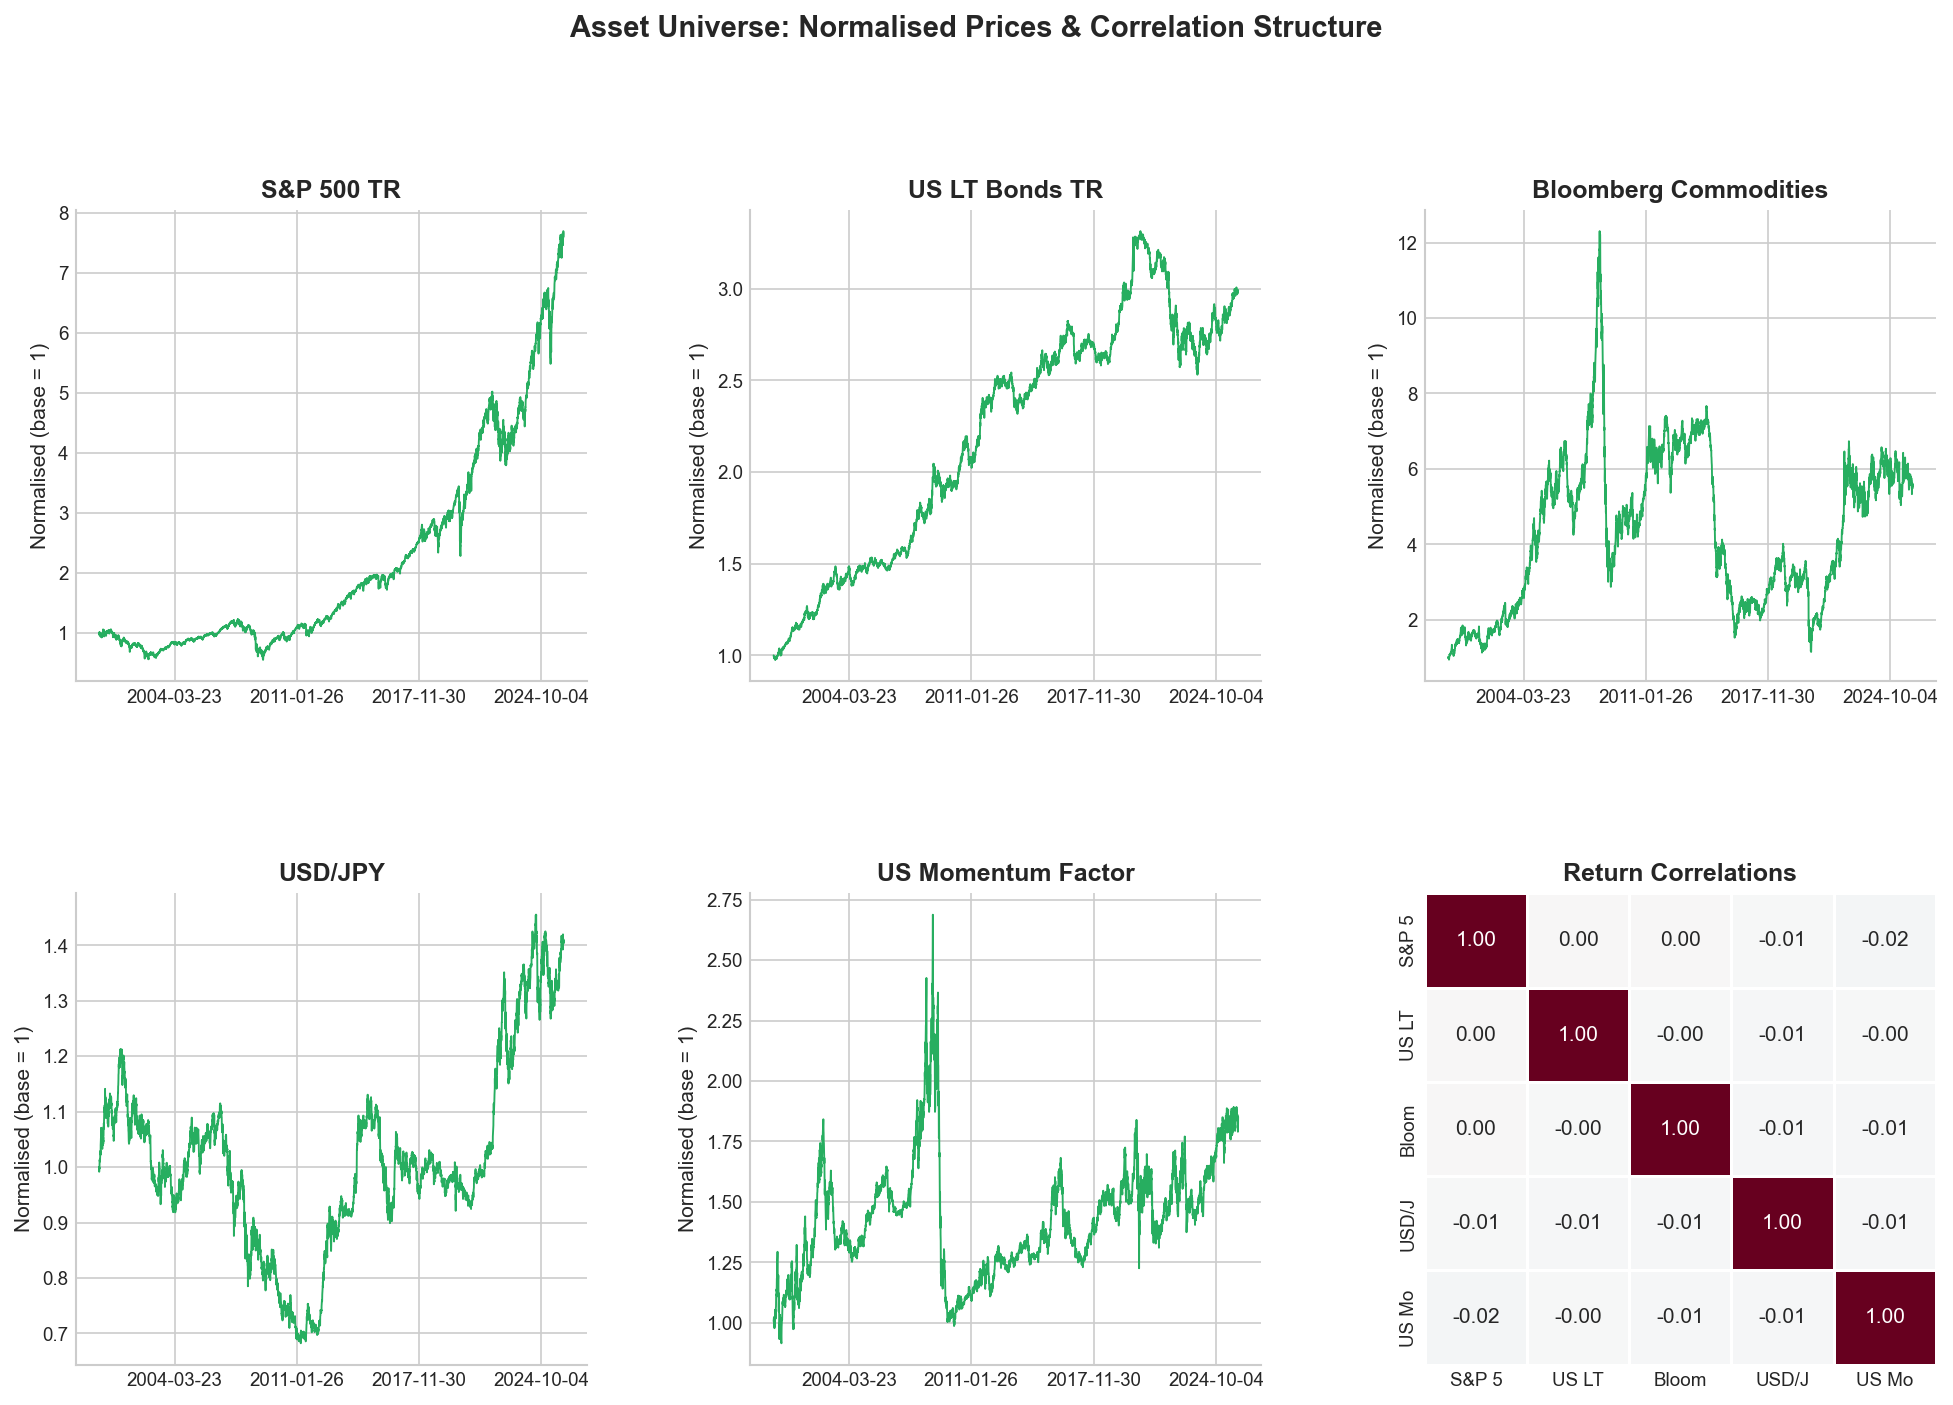
\includegraphics[width=0.92\textwidth]{fig_01_data_overview.png}
\caption{Normalised prices (base $=1$) and pairwise return correlations across the five
assets, January 2000 to December 2025.}
\label{fig:data-overview}
\end{figure}

%% ====================================================================
\section{Methodology}

\subsection{Implementation Choices}

Table~\ref{tab:implchoices} summarises the key design choices. The 48-month warm-up
ensures reliable GARCH estimation and a meaningful expanding-window target. Transaction
costs are 10~bps one-way at baseline, applied as $r^{\mathrm{net}}_t = r^{vm}_t - |\Delta w_t|\cdot c$,
consistent with the institutional estimates of \citet{frazzini2018}.

\begin{table}[H]
\centering
\small
\caption{Implementation Choices for the Volatility-Targeting Strategy}
\label{tab:implchoices}
\begin{tabularx}{\textwidth}{llX}
\toprule
\textbf{Parameter} & \textbf{Value or Rule} & \textbf{Rationale}\\
\midrule
Target volatility $\stgt$ & Expanding window, std of daily returns up to end of month $t-1$ & No look-ahead bias \citep{bongaerts2020}\\
Scaling constant $k$    & $1$ (no ex-post rescaling)                & Real-time implementable\\
Leverage cap $w_{\max}$ & $2.0$ (baseline)                          & Institutional constraint\\
Transaction cost        & 10~bps one-way (baseline)                 & \citet{frazzini2018}\\
Return frequency        & Monthly (compounded from daily)           & Avoids monthly-return bias\\
Minimum estimation window & 48 months                               & Reliable GARCH estimation\\
\bottomrule
\end{tabularx}
\end{table}

\subsection{Volatility Forecasting Models}

We implement four monthly forecasts, all strictly backward-looking. The
\textbf{one-month realised volatility} is the equally-weighted annualised standard
deviation of daily returns in month $t-1$:
$\shat^{\mathrm{RV1M}}_{i,t} = \sqrt{252/n_{t-1}\sum_{s\in t-1} r_{i,s}^2}$. The
\textbf{six-month realised volatility} uses the same expression over months $t-6$ to
$t-1$. The longer window reduces noise at the cost of slower reaction to regime shifts.
The \textbf{GJR-GARCH(1,1)} of \citet{glosten1993} captures the leverage effect:
\begin{equation}
\sigma_{i,t}^2 = \omega + \alpha r_{i,t-1}^2 + \gamma r_{i,t-1}^2 \mathbf{1}_{[r_{i,t-1}<0]} + \beta\sigma_{i,t-1}^2,
\quad \varepsilon_{i,t}\sim t_\nu,
\end{equation}
with $\gamma>0$ controlling the asymmetric impact of negative shocks. The monthly forecast
averages 21 daily variance forecasts. The \textbf{EGARCH(1,1)} of \citet{nelson1991}
operates on log-variance, eliminating non-negativity constraints and allowing sign
asymmetry independently of magnitude. Both GARCH models are re-estimated each month by
quasi-maximum likelihood on an expanding daily window, with Student-$t$ errors.

\subsection{Forecast and Performance Evaluation}

\textbf{Forecast evaluation.} We report RMSE, MAE, MAPE, the Pearson correlation between
forecast and realised volatility, and the Mincer-Zarnowitz regression
$\sigma^{\mathrm{realised}}_{i,t+1} = \alpha + \beta\,\shat_{i,t} + u_{t+1}$, with the
$F$-test of the joint null $\alpha=0$, $\beta=1$ identifying biased forecasts. Pairwise
comparisons use the \citet{diebold1995} test with squared-error loss and a Newey-West
variance correction.

\textbf{Performance evaluation.} Performance statistics are computed on monthly compounded
returns and include annualised return and volatility, the Sharpe and Sortino ratios, the
maximum drawdown, the longest drawdown duration and recovery time, the 5\% expected
shortfall, annualised turnover, CAPM alpha and beta against each asset's own Buy and Hold,
and the information and appraisal ratios. The CAPM alpha is a within-asset measure of the
abnormal return of the volatility-managed variant relative to the unmanaged variant of the
same asset; for the S\&P 500 and the momentum factor we augment this with Fama-French
three-factor and five-factor regressions (Section~6.3).

\textbf{Sharpe ratio significance.} We use two complementary tests. The first is the
Jobson-Korkie test with the \citet{memmel2003} correction, valid under IID jointly normal
returns:
\begin{equation}
z = \frac{\widehat{SR}_1 - \widehat{SR}_2}{\sqrt{\hat\theta/T}},
\quad
\hat\theta = 2(1-\hat\rho) + \tfrac{1}{2}\bigl(\widehat{SR}_1^2 + \widehat{SR}_2^2 - 2\widehat{SR}_1\widehat{SR}_2\hat\rho^2\bigr),
\end{equation}
where $\widehat{SR}_j$ is the sample monthly Sharpe of strategy $j$ and $\hat\rho$ the
sample correlation of the two excess return series. The second is a circular block
bootstrap in the spirit of \citet{ledoit2008}: $B=2{,}000$ resamples, six-month blocks,
with the two-sided $p$-value computed from the bootstrap distribution centred at the
observed Sharpe difference, and a 95\% percentile confidence interval reported. The
bootstrap is robust to autocorrelation and fat tails, both of which are present in monthly
volatility-managed returns.

%% ====================================================================
\section{Volatility Forecast Evaluation}

\begin{table}[H]
\centering
\footnotesize
\caption{Volatility Forecast Evaluation: Error Metrics, Correlation, Mincer-Zarnowitz}
\label{tab:fc-eval}
\begin{tabular}{llrrrrrrr}
\toprule
\textbf{Asset} & \textbf{Model} & \textbf{RMSE} & \textbf{MAE} & \textbf{MAPE} & \textbf{Corr.} & $\hat\alpha$ & $\hat\beta$ & $R^2$\\
\midrule
\multirow{4}{*}{S\&P 500 TR}
& RV 1M       & 0.089 & 0.054 & 0.368 & 0.648 & 0.053 & 0.648 & 0.420\\
& RV 6M       & 0.103 & 0.061 & 0.441 & 0.479 & 0.060 & 0.559 & 0.229\\
& GJR-GARCH   & \textbf{0.074} & 0.049 & 0.374 & \textbf{0.737} & 0.009 & 0.875 & \textbf{0.544}\\
& EGARCH      & 0.075 & 0.049 & 0.371 & 0.713 & $-0.017$ & 1.072 & 0.509\\
\midrule
\multirow{4}{*}{US LT Bonds TR}
& RV 1M       & 0.021 & 0.014 & 0.234 & 0.605 & 0.024 & 0.606 & 0.366\\
& RV 6M       & 0.020 & 0.014 & 0.248 & 0.623 & 0.013 & 0.743 & 0.389\\
& GJR-GARCH   & 0.019 & 0.013 & 0.233 & 0.649 & 0.008 & 0.820 & 0.421\\
& EGARCH      & \textbf{0.018} & 0.013 & 0.226 & \textbf{0.670} & 0.003 & 0.895 & \textbf{0.449}\\
\midrule
\multirow{4}{*}{Bloomberg Comm.}
& RV 1M       & 0.127 & 0.085 & 0.287 & 0.637 & 0.108 & 0.637 & 0.406\\
& RV 6M       & 0.142 & 0.093 & 0.329 & 0.481 & 0.113 & 0.583 & 0.231\\
& GJR-GARCH   & 0.123 & 0.088 & 0.326 & 0.620 & 0.043 & 0.779 & 0.385\\
& EGARCH      & \textbf{0.116} & 0.083 & 0.307 & \textbf{0.649} & 0.000 & 0.928 & \textbf{0.422}\\
\midrule
\multirow{4}{*}{USD/JPY}
& RV 1M       & 0.037 & 0.027 & 0.312 & 0.514 & 0.042 & 0.514 & 0.264\\
& RV 6M       & 0.035 & 0.027 & 0.330 & 0.481 & 0.029 & 0.628 & 0.232\\
& GJR-GARCH   & 0.033 & 0.026 & 0.337 & \textbf{0.546} & 0.012 & 0.787 & \textbf{0.298}\\
& EGARCH      & \textbf{0.033} & 0.025 & 0.325 & 0.532 & 0.005 & 0.879 & 0.283\\
\midrule
\multirow{4}{*}{US Momentum}
& RV 1M       & 0.054 & 0.038 & 0.303 & 0.810 & 0.025 & 0.810 & 0.656\\
& RV 6M       & 0.066 & 0.043 & 0.384 & 0.707 & 0.025 & 0.767 & 0.500\\
& GJR-GARCH   & \textbf{0.052} & 0.036 & 0.306 & \textbf{0.821} & 0.011 & 0.903 & \textbf{0.675}\\
& EGARCH      & 0.052 & 0.036 & 0.307 & 0.817 & 0.012 & 0.890 & 0.668\\
\bottomrule
\end{tabular}
\end{table}

\noindent\textit{Notes:} Best performer per asset highlighted in bold. The Mincer-Zarnowitz
$F$-test rejects the joint null $\hat\alpha=0$, $\hat\beta=1$ at $p<0.05$ for RV 1M and
RV 6M on every asset, and for GJR-GARCH on every asset except the S\&P 500, where EGARCH
is the only model that fails to reject ($p=0.241$).

\textbf{GJR-GARCH dominates on equities and momentum.} For the S\&P 500, GJR-GARCH reduces
RMSE by 17.5\% relative to RV 1M and raises $R^2$ from 0.42 to 0.54. The Mincer-Zarnowitz
slope ($\hat\beta=0.875$) is closer to the ideal value of one than that of RV 1M
($\hat\beta=0.648$). The leverage-effect parameter $\gamma>0$ is the likely source, as
equities exhibit strong asymmetric volatility responses to negative returns.

\textbf{EGARCH is the best model for bonds, commodities, and FX.} EGARCH achieves the
lowest RMSE for US long-term bonds (0.018), Bloomberg Commodities (0.116), and USD/JPY
(0.033). Its Mincer-Zarnowitz slope is the closest to one for these three assets.

\textbf{RV 6M is systematically biased.} Across every asset, RV 6M displays the highest
RMSE and the lowest $R^2$, with Mincer-Zarnowitz slopes between 0.56 and 0.74, indicating
severe underestimation during volatility spikes. Despite these deficiencies, RV 6M achieves
competitive portfolio performance through its low turnover (Section~7).

\textbf{Momentum is the most forecastable asset} (GJR-GARCH $R^2=0.675$), reflecting the
prolonged variance bursts that accompany momentum crashes. \textbf{USD/JPY shows the
weakest forecastability} ($R^2<0.30$ for every model), consistent with the near-random-walk
behaviour of spot exchange rates \citep{meese1983}. Diebold-Mariano pairwise tests find
no statistically significant accuracy difference between GJR-GARCH and EGARCH at the 5\%
level on any asset; both significantly outperform RV 1M for equities.

\begin{figure}[H]
\centering
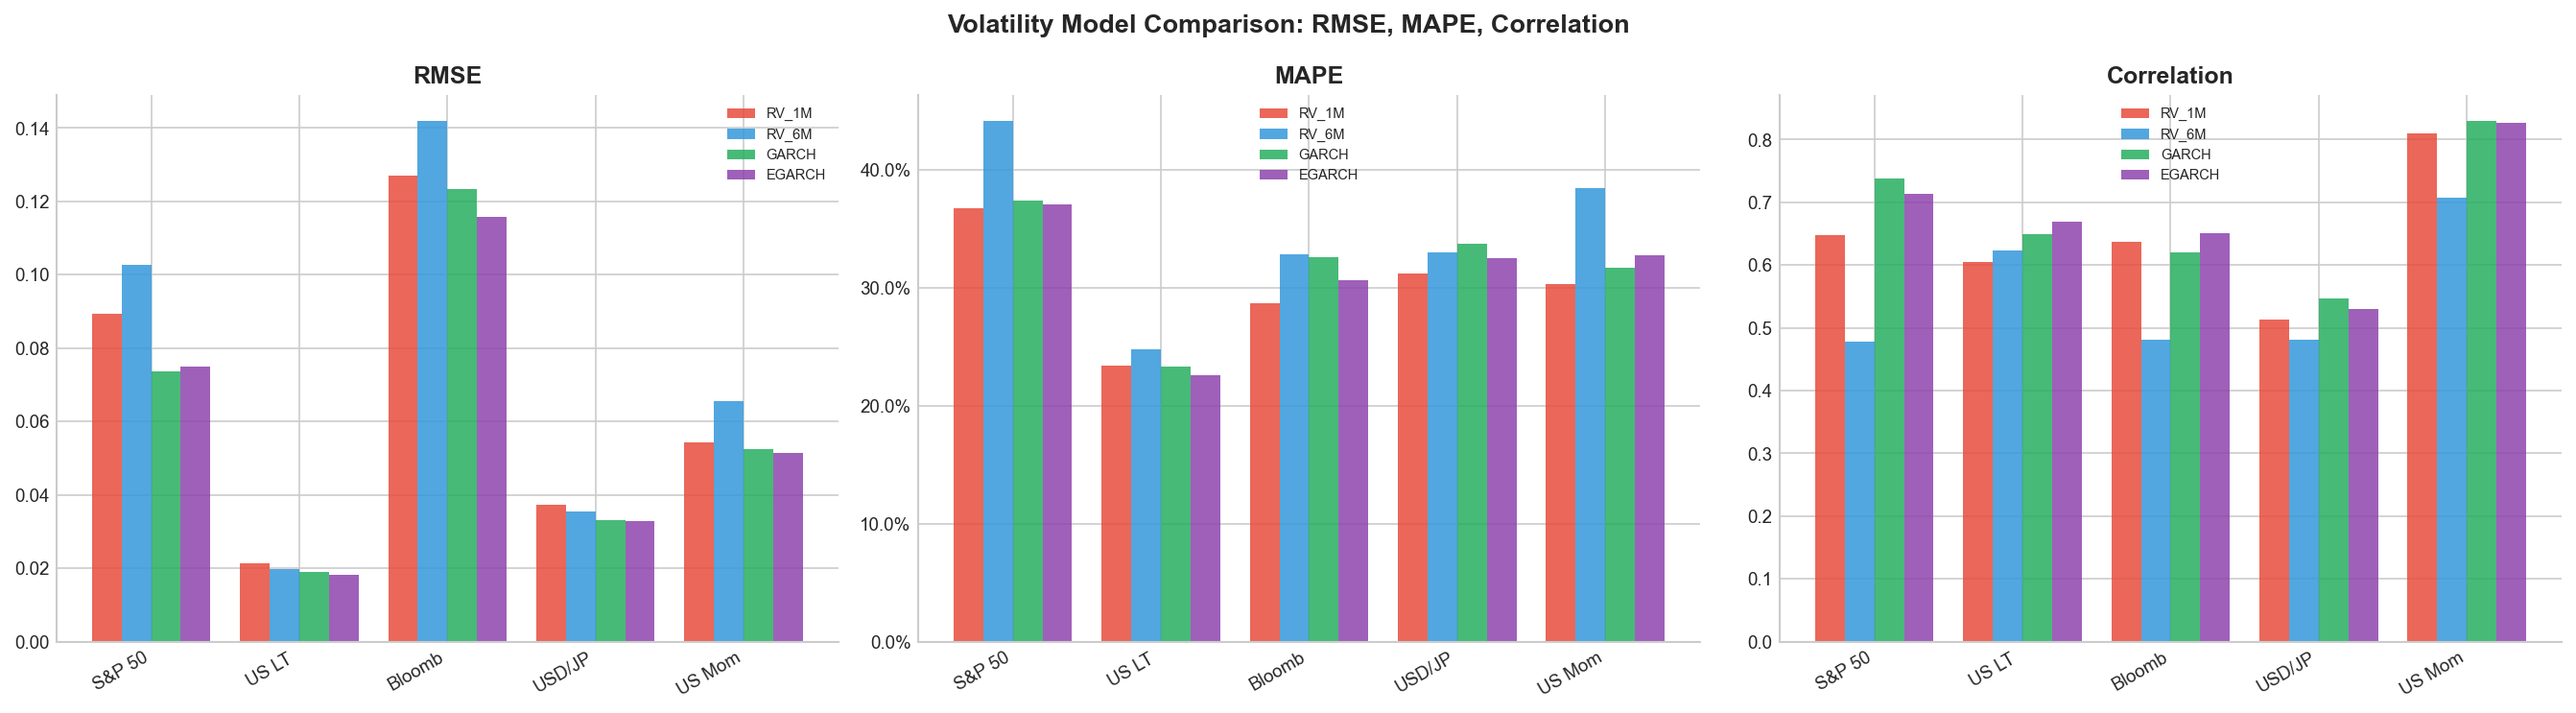
\includegraphics[width=0.86\textwidth]{fig_03_forecast_bar.png}
\caption{Volatility Model Comparison: RMSE, MAPE, and Correlation. GJR-GARCH and EGARCH
dominate the realised-volatility benchmarks for equities and momentum; improvements for FX
and commodities are smaller.}
\label{fig:fc-bar}
\end{figure}

%% ====================================================================
\section{Implementation Diagnostics}

\subsection{Realised versus Target Volatility, and the Constant $k$}

A volatility-targeting strategy with $k=1$ does not, in general, deliver a realised
volatility equal to the target; the ratio is informative about the unbiasedness of the
volatility forecast. In our sample, the realised-to-target ratio lies between 0.94 and
1.05 for fifteen of the twenty volatility-managed entries, indicating that $k=1$ is
operationally reasonable. The largest deviations are a ratio of 0.82 for the two GARCH
variants on the S\&P 500 (slightly too defensive) and a ratio of 1.19 for VM RV 1M on
USD/JPY (the strategy runs hot because RV 1M underestimates FX volatility). The ex-post
implied scaling constant $k^*=\stgt/\mathrm{Vol}(r/\shat)$ is between 1.12 and 1.22 for the
S\&P 500 and close to one for the other assets, but it uses information from the entire
sample and is therefore inadmissible for real-time deployment; we retain $k=1$ throughout
and report $k^*$ only as a diagnostic.

\subsection{Empirical Cost of the Look-Ahead Bias}

To quantify the magnitude of the bias, we recompute every volatility-managed strategy
under both the expanding-window estimator of Equation~(\ref{eq:target}) and the
look-ahead-biased full-sample estimator used by \citet{moreira2017} and \citet{harvey2018}.
Table~\ref{tab:bias} reports the impact on annualised Sharpe ratios.

\begin{table}[H]
\centering
\footnotesize
\caption{Impact of the Look-Ahead Bias on Annualised Sharpe Ratios}
\label{tab:bias}
\begin{tabular}{llrrrr}
\toprule
\textbf{Asset} & \textbf{Strategy} & \textbf{SR biased} & \textbf{SR unbiased} & $\Delta$ Sharpe & \textbf{Inflation}\\
\midrule
S\&P 500 TR     & VM RV 1M     & 0.781 & 0.809 & $-0.028$ & $-3.4\%$\\
                & VM GJR-GARCH & 0.757 & 0.785 & $-0.027$ & $-3.5\%$\\
US LT Bonds     & VM GJR-GARCH & 0.255 & 0.256 & $-0.001$ & $-0.4\%$\\
Bloomberg Comm. & VM GJR-GARCH & 0.147 & 0.162 & $-0.015$ & $-9.2\%$\\
USD/JPY         & VM GJR-GARCH & 0.109 & 0.116 & $-0.007$ & $-6.1\%$\\
US Momentum     & VM GJR-GARCH & 0.385 & 0.363 & $+0.022$ & $+6.1\%$\\
\bottomrule
\end{tabular}
\end{table}

\noindent The average bias-induced inflation across all twenty volatility-managed cells in
our sample is $-2.4\%$. For the S\&P 500, the bias actually reduces (rather than inflates)
the Sharpe ratio, the opposite of the direction emphasised by \citet{liu2019}. The intuition
is that the expanding-window target starts at its value at the end of the 48-month warm-up
window, which on the S\&P 500 over 2000--2003 was a high-volatility regime (the dot-com
crash); the initial values of $\stgt_t$ are therefore higher than the eventual full-sample
standard deviation, the strategy levers up more aggressively in the early years, and the
resulting Sharpe ratio is slightly higher. The largest absolute bias is on commodities and
USD/JPY, the two assets for which forecast quality is the weakest. In aggregate the
bias is smaller in our sample than \citet{liu2019} document for the US equity factor
universe, but only the expanding-window specification is admissible for real-time
deployment.

%% ====================================================================
\section{Performance Evaluation}

\subsection{Full-Sample Performance}

Table~\ref{tab:perf-all} reports the full-sample performance statistics for the five
assets at the baseline of 10~bps transaction cost and a 200\% leverage cap.
Figure~\ref{fig:cumret} plots the cumulative wealth paths.

\begin{table}[H]
\centering
\footnotesize
\caption{Full-Sample Performance by Asset and Strategy (TC $=$ 10~bps, Leverage cap $=$ 200\%)}
\label{tab:perf-all}
\begin{tabular}{llrrrrrrr}
\toprule
\textbf{Asset} & \textbf{Strategy} & \textbf{Ret} & \textbf{Vol} & \textbf{Sharpe} & \textbf{Sortino} & \textbf{MaxDD} & \textbf{DDdur (m)} & \textbf{TO}\\
\midrule
\multirow{5}{*}{S\&P 500}
& Buy and Hold   & 10.7\% & 14.6\% & 0.658 & 0.871 & $-50.9\%$ & 52 & 0.00\\
& VM RV 1M       & 15.6\% & 17.9\% & 0.809 & 1.231 & $-39.3\%$ & 42 & 3.73\\
& VM RV 6M       & 13.4\% & 17.5\% & 0.713 & 1.028 & $-37.4\%$ & 44 & 1.13\\
& VM GJR-GARCH   & 14.1\% & 16.5\% & 0.785 & 1.193 & $-36.8\%$ & 40 & 3.88\\
& VM EGARCH      & 13.7\% & 16.5\% & 0.762 & 1.147 & $-40.6\%$ & 42 & 3.68\\
\midrule
\multirow{5}{*}{US LT Bonds}
& Buy and Hold   & 3.4\% & 6.4\% & 0.294 & 0.426 & $-22.2\%$ & 66 & 0.00\\
& VM RV 1M       & 2.9\% & 7.0\% & 0.193 & 0.277 & $-23.0\%$ & 66 & 3.06\\
& VM RV 6M       & 3.4\% & 6.6\% & 0.278 & 0.417 & $-20.9\%$ & 66 & 0.68\\
& VM GJR-GARCH   & 3.2\% & 6.4\% & 0.256 & 0.378 & $-21.1\%$ & 66 & 1.19\\
& VM EGARCH      & 3.1\% & 6.4\% & 0.236 & 0.346 & $-21.6\%$ & 66 & 1.19\\
\midrule
\multirow{5}{*}{Commodities}
& Buy and Hold   & 3.7\% & 32.9\% & 0.235 & 0.315 & $-88.5\%$ & 211 & 0.00\\
& VM RV 1M       & 0.8\% & 38.0\% & 0.175 & 0.244 & $-91.1\%$ & 165 & 3.50\\
& VM RV 6M       & 2.0\% & 34.7\% & 0.193 & 0.256 & $-90.2\%$ & 211 & 0.78\\
& VM GJR-GARCH   & 1.3\% & 32.9\% & 0.162 & 0.225 & $-88.3\%$ & 211 & 1.78\\
& VM EGARCH      & 1.3\% & 33.2\% & 0.162 & 0.227 & $-88.9\%$ & 211 & 1.78\\
\midrule
\multirow{5}{*}{USD/JPY}
& Buy and Hold   & 1.6\% &  9.8\% & 0.040 & 0.060 & $-37.1\%$ & 97 & 0.00\\
& VM RV 1M       & 2.0\% & 11.7\% & 0.085 & 0.137 & $-39.8\%$ & 96 & 3.83\\
& VM RV 6M       & 2.7\% & 10.9\% & 0.142 & 0.238 & $-36.4\%$ & 94 & 0.92\\
& VM GJR-GARCH   & 2.4\% & 10.2\% & 0.116 & 0.194 & $-35.4\%$ & 94 & 1.66\\
& VM EGARCH      & 2.2\% & 10.3\% & 0.099 & 0.164 & $-36.9\%$ & 96 & 1.68\\
\midrule
\multirow{5}{*}{Momentum}
& Buy and Hold   & 1.5\% & 15.0\% & 0.066 & 0.076 & $-61.0\%$ & 205 & 0.00\\
& VM RV 1M       & 6.6\% & 17.5\% & 0.356 & 0.524 & $-43.1\%$ &  79 & 2.80\\
& VM RV 6M       & 7.2\% & 16.5\% & 0.400 & 0.624 & $-35.5\%$ &  60 & 0.80\\
& VM GJR-GARCH   & 6.5\% & 16.2\% & 0.363 & 0.561 & $-38.4\%$ &  73 & 2.42\\
& VM EGARCH      & 6.3\% & 15.9\% & 0.357 & 0.558 & $-38.9\%$ &  73 & 2.35\\
\bottomrule
\end{tabular}
\end{table}

\begin{figure}[H]
\centering
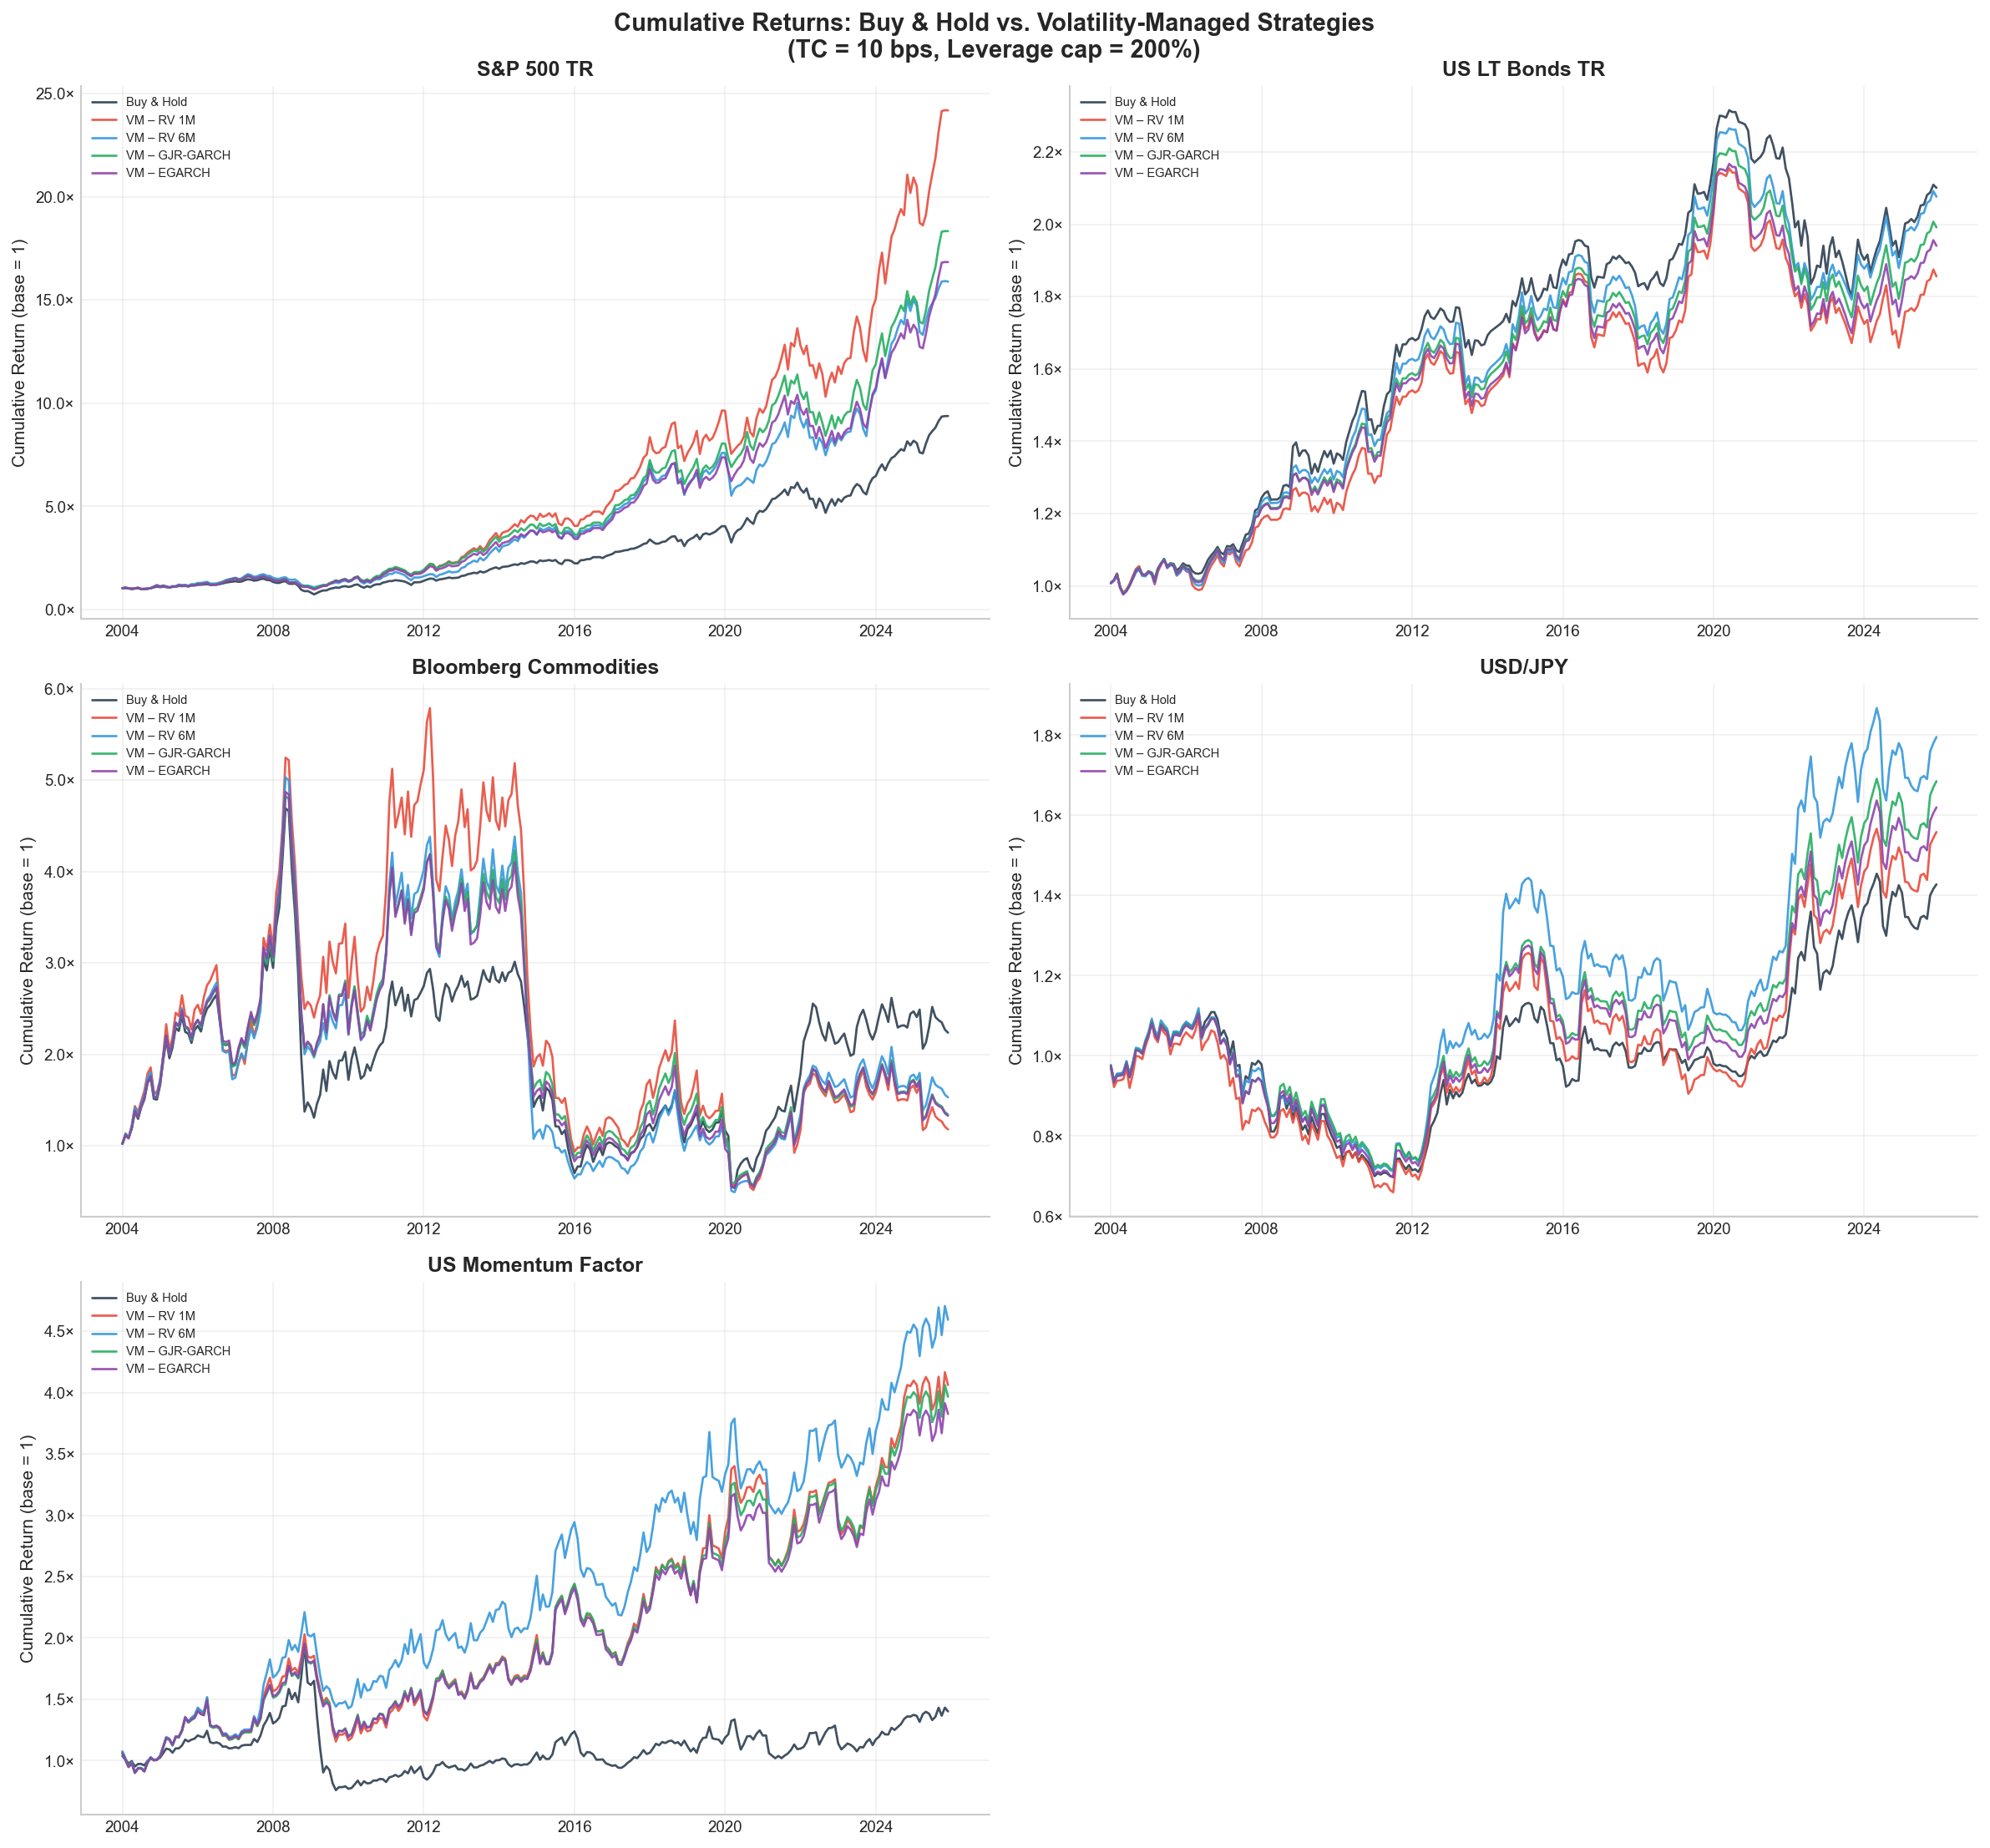
\includegraphics[width=0.92\textwidth]{fig_04_cumulative_returns.png}
\caption{Cumulative Returns: Buy and Hold versus Volatility-Managed Strategies (TC $=$ 10~bps,
leverage cap $=$ 200\%).}
\label{fig:cumret}
\end{figure}

\subsection{Statistical Significance of Sharpe Ratio Differences}

Table~\ref{tab:sigtest} reports the Jobson-Korkie-Memmel and block-bootstrap tests of every
(volatility-managed strategy minus Buy and Hold) pair, and the GJR-GARCH versus EGARCH
model comparison.

\begin{table}[H]
\centering
\footnotesize
\caption{Sharpe Ratio Significance Tests (VM strategies vs.\ Buy and Hold; selected pairs)}
\label{tab:sigtest}
\begin{tabular}{llrrrrr}
\toprule
\textbf{Asset} & \textbf{Pair} & $\Delta$ SR & \textbf{JKM} $z$ & \textbf{JKM} $p$ & \textbf{Boot} $p$ & \textbf{Boot 95\% CI}\\
\midrule
\multirow{4}{*}{S\&P 500}
& VM RV 1M vs.\ B\&H     & $+0.151$ & $+1.53$ & 0.125 & 0.208 & $[-0.07,+0.38]$\\
& VM RV 6M vs.\ B\&H     & $+0.055$ & $+0.63$ & 0.529 & 0.660 & $[-0.18,+0.28]$\\
& VM GJR-GARCH vs.\ B\&H & $+0.126$ & $+1.31$ & 0.191 & 0.301 & $[-0.10,+0.35]$\\
& VM EGARCH vs.\ B\&H    & $+0.104$ & $+1.17$ & 0.240 & 0.332 & $[-0.10,+0.31]$\\
\midrule
US LT Bonds
& VM GJR-GARCH vs.\ B\&H & $-0.037$ & $-0.62$ & 0.533 & 0.517 & $[-0.15,+0.07]$\\
\midrule
Commodities
& VM GJR-GARCH vs.\ B\&H & $-0.073$ & $-1.05$ & 0.292 & 0.306 & $[-0.21,+0.06]$\\
\midrule
USD/JPY
& VM GJR-GARCH vs.\ B\&H & $+0.076$ & $+1.42$ & 0.155 & 0.192 & $[-0.04,+0.19]$\\
\midrule
\multirow{4}{*}{Momentum}
& VM RV 1M vs.\ B\&H     & $+0.290^{**}$  & $+2.68$ & 0.007 & 0.015 & $[+0.06,+0.52]$\\
& VM RV 6M vs.\ B\&H     & $+0.334^{***}$ & $+3.15$ & 0.002 & 0.003 & $[+0.10,+0.55]$\\
& VM GJR-GARCH vs.\ B\&H & $+0.297^{**}$  & $+2.70$ & 0.007 & 0.013 & $[+0.05,+0.53]$\\
& VM EGARCH vs.\ B\&H    & $+0.291^{**}$  & $+2.75$ & 0.006 & 0.012 & $[+0.06,+0.52]$\\
\bottomrule
\end{tabular}
\end{table}

\noindent\textit{Notes:} Significance $^*p<0.10$, $^{**}p<0.05$, $^{***}p<0.01$, using the more
conservative of the two $p$-values. Bootstrap: $B=2{,}000$ resamples, six-month blocks.

\noindent The headline finding is that, on conventional statistical criteria, the Sharpe
ratio improvement is significant only for the momentum factor. All four momentum pairs
reach $p<0.05$ on both tests, with bootstrap confidence intervals comfortably above zero.
For the other four assets, the bootstrap confidence intervals all contain zero. The S\&P
500 GJR-GARCH versus Buy and Hold point estimate is $+0.126$ with a 95\% interval of
$[-0.10,+0.35]$: economically meaningful but not statistically distinguishable from zero
at conventional levels. This pattern is exactly the one anticipated by \citet{liu2019}.
The GJR-GARCH versus EGARCH model comparison shows no statistically significant difference
on any asset except US LT bonds, where GJR-GARCH outperforms by $0.020$ in Sharpe; too
small for practical relevance.

\subsection{Fama-French Alpha Regressions}

For the S\&P 500 and the momentum factor, we run alpha regressions on the Fama-French
three- and five-factor models:
\begin{equation}
r^{exc}_{i,t} = \alpha_i + \beta^{\mathrm{MKT}}_i \mathrm{MKT}_t + \beta^{\mathrm{SMB}}_i \mathrm{SMB}_t
+ \beta^{\mathrm{HML}}_i \mathrm{HML}_t \bigl[+ \beta^{\mathrm{RMW}}_i \mathrm{RMW}_t + \beta^{\mathrm{CMA}}_i \mathrm{CMA}_t\bigr] + u_{i,t},
\end{equation}
with Newey-West HAC standard errors (six lags). The bracketed terms are present in the
five-factor specification only. For the momentum factor, we exclude the momentum factor
from the right-hand side; the resulting alpha measures the value added by volatility-managing
momentum on top of static equity-style exposures. We do not run Fama-French regressions
for bonds, commodities, or FX because the Fama-French factors are designed to span the
equity-return generating process; a proper multi-factor risk model for these assets would
involve term and default factors, commodity carry and momentum factors, and FX carry and
value factors. We acknowledge this as a limitation.

\begin{table}[H]
\centering
\footnotesize
\caption{Fama-French Alpha Regressions (Newey-West HAC, 6 lags)}
\label{tab:ff}
\begin{tabular}{lllrrrr}
\toprule
\textbf{Asset} & \textbf{Strategy} & \textbf{Model} & $\alpha$ \textbf{(ann.)} & $t(\alpha)$ & $p(\alpha)$ & \textbf{Adj.\ }$R^2$\\
\midrule
\multirow{6}{*}{S\&P 500}
& Buy and Hold   & FF3 & $-0.22\%$       & $-0.98$ & 0.328 & 0.997\\
& Buy and Hold   & FF5 & $-0.41\%^{**}$  & $-2.15$ & 0.032 & 0.997\\
& VM RV 1M       & FF3 & $+3.54\%^{*}$   & $+1.74$ & 0.081 & 0.803\\
& VM GJR-GARCH   & FF3 & $+2.77\%$       & $+1.51$ & 0.132 & 0.813\\
& VM GJR-GARCH   & FF5 & $+2.81\%$       & $+1.58$ & 0.115 & 0.815\\
& VM EGARCH      & FF3 & $+2.27\%$       & $+1.39$ & 0.163 & 0.838\\
\midrule
\multirow{6}{*}{Momentum}
& Buy and Hold   & FF3 & $+3.57\%$       & $+1.22$ & 0.224 & 0.179\\
& Buy and Hold   & FF5 & $+2.99\%$       & $+0.94$ & 0.348 & 0.211\\
& VM RV 1M       & FF3 & $+8.33\%^{**}$  & $+2.53$ & 0.011 & 0.124\\
& VM RV 6M       & FF3 & $+8.73\%^{***}$ & $+2.81$ & 0.005 & 0.104\\
& VM GJR-GARCH   & FF3 & $+7.76\%^{**}$  & $+2.52$ & 0.012 & 0.122\\
& VM EGARCH      & FF3 & $+7.49\%^{**}$  & $+2.47$ & 0.014 & 0.120\\
\bottomrule
\end{tabular}
\end{table}

For the S\&P 500, alpha point estimates are between $+1.5\%$ and $+3.5\%$ per year, but
only the RV 1M alpha reaches marginal significance ($p=0.08$). For the momentum factor,
every volatility-managed alpha is between $+7.5\%$ and $+8.7\%$ with $t>2.3$, all
significant at the 5\% level. The market beta on the momentum variants is consistently
negative ($\hat\beta^{\mathrm{MKT}}\approx -0.20$), reflecting the long-short construction,
and the adjusted $R^2$ is low ($\approx 0.12$), confirming that the volatility management
of momentum is a genuine timing skill rather than a tilt towards a static factor exposure.

\subsection{Multi-Asset Equal-Weight Portfolio}

The near-zero cross-asset correlations documented in Section~2 suggest that combining the
volatility-managed strategies should deliver diversification benefits on top of within-asset
timing. Table~\ref{tab:multi} reports the performance of an equal-weight portfolio of the
five GJR-GARCH or EGARCH variants, rebalanced monthly, against the equal-weight Buy and
Hold benchmark on the same five assets.

\begin{table}[H]
\centering
\small
\caption{Multi-Asset Equal-Weight Portfolios (TC $=$ 10~bps)}
\label{tab:multi}
\begin{tabular}{lrrrrrr}
\toprule
\textbf{Strategy} & \textbf{Ann.\ Ret} & \textbf{Ann.\ Vol} & \textbf{Sharpe} & \textbf{Sortino} & \textbf{MaxDD} & \textbf{ES(5\%)}\\
\midrule
EW Buy and Hold     & 5.68\% & 7.52\% & 0.548 & 0.762 & $-25.9\%$ & $-4.56\%$\\
EW VM GJR-GARCH     & 7.00\% & 8.03\% & 0.673 & 1.026 & $-19.5\%$ & $-4.68\%$\\
EW VM EGARCH        & 6.81\% & 8.09\% & 0.646 & 0.984 & $-19.8\%$ & $-4.78\%$\\
\bottomrule
\end{tabular}
\end{table}

\noindent The equal-weight GJR-GARCH portfolio achieves a Sharpe ratio of 0.673, higher
than every single-asset volatility-managed Sharpe in Table~\ref{tab:perf-all} except for
momentum (where the long-short construction is not directly comparable). The maximum
drawdown is reduced by 6.4 percentage points (from 25.9\% to 19.5\%), while expected
shortfall is essentially unchanged. Volatility timing and cross-asset diversification stack
rather than substitute.

\subsection{Discussion by Asset}

\textbf{S\&P 500.} GJR-GARCH raises the Sharpe ratio from 0.658 to 0.785 (a 19\% increase),
reduces the maximum drawdown from 50.9\% to 36.8\%, and cuts the recovery time from 37 to
20 months. The Sortino ratio improves from 0.871 to 1.193, indicating that the improvement
comes from a reduction in downside risk. However, neither the Sharpe difference
($p=0.30$ bootstrap, 95\% CI $[-0.10,+0.35]$) nor the FF3/FF5 alpha ($p=0.13$) is statistically
significant: the economic case is suggestive, the statistical case is weaker.

\textbf{US LT Bonds.} Volatility management modestly destroys value (Sharpe 0.256 vs.\ 0.294
under GJR-GARCH). The mechanism is the flight-to-quality dynamic: bond volatility rises in
equity-market crises, when bonds typically generate positive returns, so the strategy
de-risks at the moments when bonds are most valuable.

\textbf{Bloomberg Commodities.} Volatility management is counterproductive
($\Delta SR=-0.073$). Two structural factors drive this result: the high base volatility
($\approx 33\%$) leaves little room to lever within the cap, and the catastrophic 88\%
drawdown from the 2008 super-cycle peak reflects fundamental price dynamics rather than
the volatility-clustering shocks that GARCH-type models anticipate.

\textbf{USD/JPY.} A modest improvement is observed ($\Delta SR=+0.076$ for GJR-GARCH).
RV 6M produces the highest Sharpe (0.142) despite GJR-GARCH dominating on forecast
accuracy, because the weak FX forecastability ($R^2<0.30$) makes the smoother,
lower-turnover RV 6M signal more economically valuable.

\textbf{US Momentum Factor.} The only asset on which the Sharpe improvement is both
economically and statistically large. The Sharpe ratio rises from 0.066 to 0.363, the
maximum drawdown shrinks from 61\% to 38\%, the longest drawdown shortens from 205 to 73
months, and the bootstrap $p$-value is 0.013. The intuition, established in
\citet{moreira2017}, is that momentum crashes occur during volatility spikes (the March
2009 reversal and the March 2020 COVID shock), so the strategy avoids them almost
mechanically.

%% ====================================================================
\section{NBER Business Cycle Analysis}

A central claim of volatility-targeting proponents is that the strategy delivers automatic
recession protection. Three NBER recessions overlap with our sample: the dot-com recession
(March--November 2001, 9 months, which falls within the 48-month warm-up window), the
Great Financial Crisis (December 2007--June 2009, 19 months), and the COVID-19 recession
(February--April 2020, 3 months). After the warm-up, the usable sample contains 22
recession months out of 264, dominated by the Great Financial Crisis.

\begin{table}[H]
\centering
\footnotesize
\caption{Performance by NBER Business Cycle Phase (Annualised)}
\label{tab:nber}
\begin{tabular}{llrrrrrr}
\toprule
& & \multicolumn{3}{c}{\textbf{Expansion (242 months)}} & \multicolumn{3}{c}{\textbf{Recession (22 months)}}\\
\cmidrule(lr){3-5}\cmidrule(lr){6-8}
\textbf{Asset} & \textbf{Strategy} & \textbf{Ret} & \textbf{Vol} & \textbf{SR} & \textbf{Ret} & \textbf{Vol} & \textbf{SR}\\
\midrule
\multirow{2}{*}{S\&P 500}     & Buy and Hold   & 14.6\% & 12.6\% & 1.16  & $-25.4\%$ & 26.5\% & $-0.96$\\
                              & VM GJR-GARCH   & 17.7\% & 16.3\% & 1.08  & $-18.6\%$ & 16.0\% & $-1.16$\\
\multirow{2}{*}{US LT Bonds}  & Buy and Hold   &  3.1\% &  6.2\% & 0.50  & $+9.0\%$  &  8.7\% & $+1.03$\\
                              & VM GJR-GARCH   &  3.0\% &  6.4\% & 0.47  & $+6.7\%$  &  5.9\% & $+1.13$\\
\multirow{2}{*}{Commodities}  & Buy and Hold   & 15.0\% & 29.0\% & 0.52  & $-52.4\%$ & 59.3\% & $-0.88$\\
                              & VM GJR-GARCH   & 10.9\% & 31.0\% & 0.35  & $-35.6\%$ & 48.6\% & $-0.73$\\
\multirow{2}{*}{USD/JPY}      & Buy and Hold   &  3.1\% &  9.4\% & 0.33  & $-8.7\%$  & 13.3\% & $-0.65$\\
                              & VM GJR-GARCH   &  3.5\% & 10.2\% & 0.35  & $-4.3\%$  & 10.4\% & $-0.41$\\
\multirow{2}{*}{Momentum}     & Buy and Hold   &  3.5\% & 12.0\% & 0.29  & $-5.7\%$  & 34.4\% & $-0.17$\\
                              & VM GJR-GARCH   &  7.5\% & 16.0\% & 0.47  & $+8.7\%$  & 19.5\% & $+0.45$\\
\bottomrule
\end{tabular}
\end{table}

\textbf{Small-sample caveat.} With $T=22$ recession months, the 95\% confidence interval
around any single recession Sharpe is roughly $\pm 0.43$; differences smaller than half a
Sharpe point are not statistically distinguishable from sampling noise. With this caveat,
the recession-loss reduction is meaningful for the S\&P 500 (6.8 percentage points),
commodities (16.8 percentage points), USD/JPY (a halving of the loss), and momentum (a
sign flip from $-5.7\%$ to $+8.7\%$). For bonds, the flight-to-quality premium is partially
sacrificed by the volatility-targeting adjustment, but the proportional volatility
compression preserves the recession Sharpe.

\begin{figure}[H]
\centering
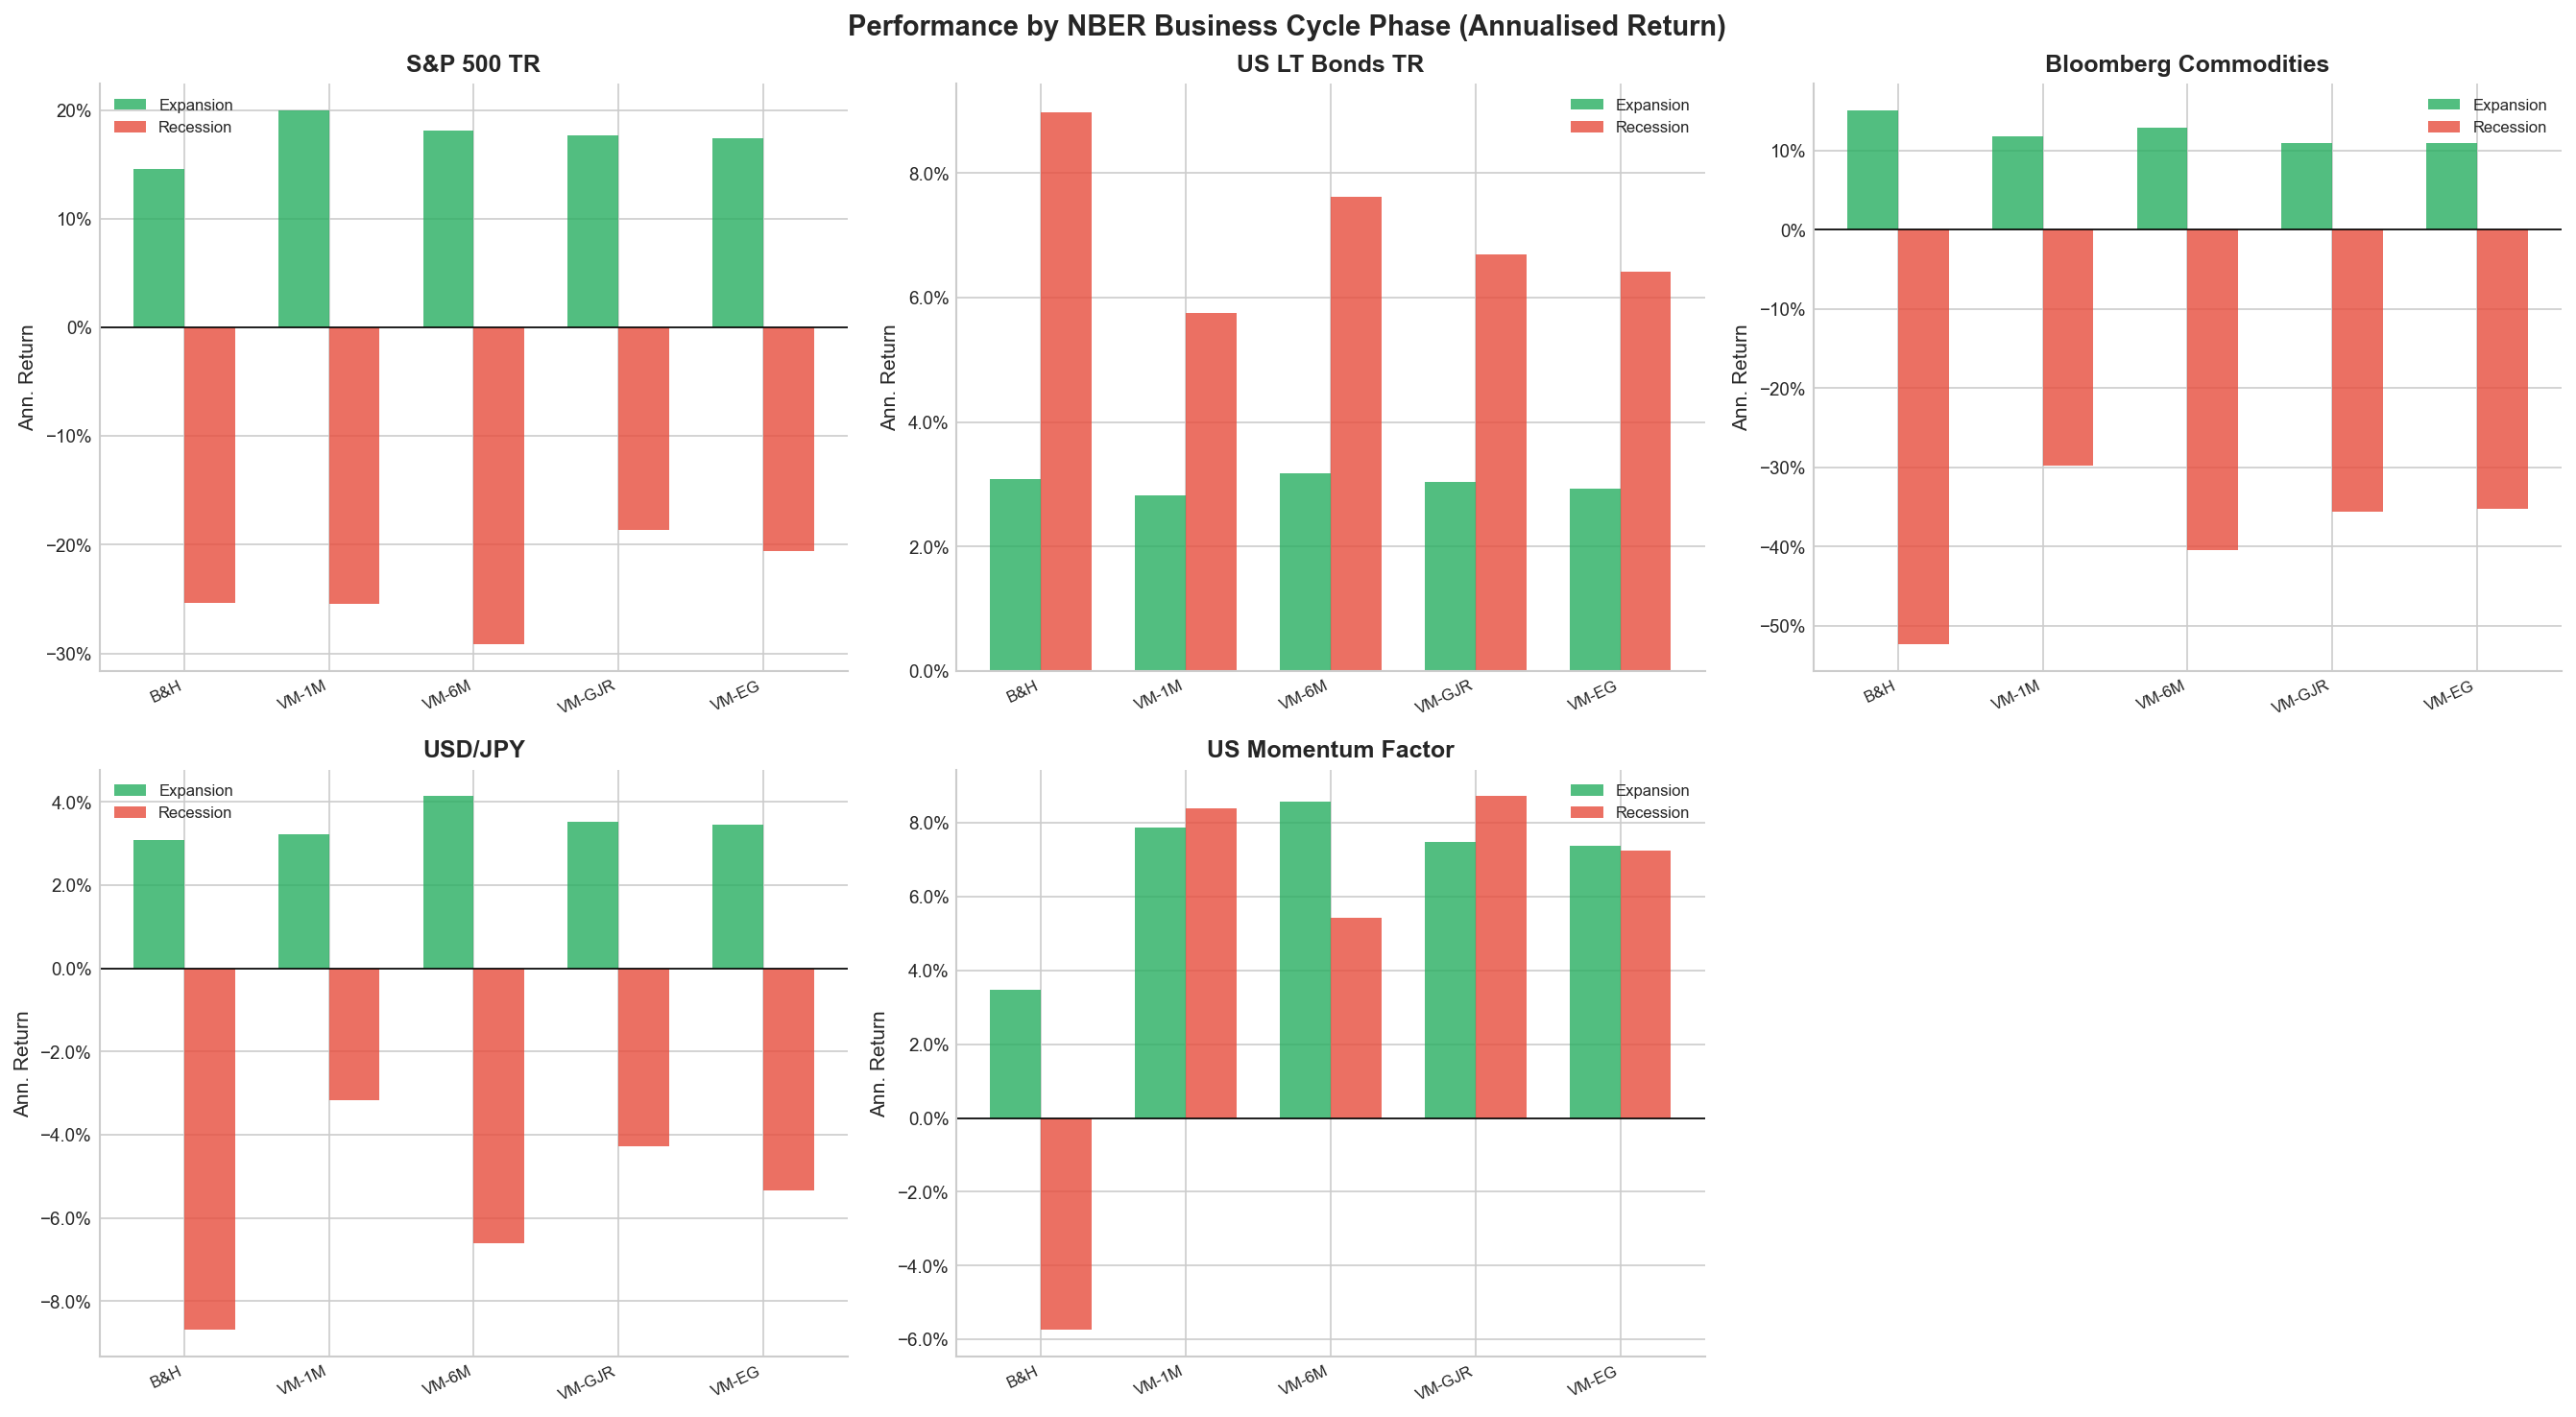
\includegraphics[width=0.92\textwidth]{fig_05_nber.png}
\caption{Annualised return by NBER business cycle phase. The volatility-managed strategies
provide meaningful loss reduction during recessions for the S\&P 500, commodities, and
momentum.}
\label{fig:nber}
\end{figure}

%% ====================================================================
\section{Transaction Costs, Turnover, and Leverage}

\subsection{Turnover and Transaction Cost Sensitivity}

\begin{table}[H]
\centering
\small
\caption{Annualised Turnover by Asset and Model}
\label{tab:turnover}
\begin{tabular}{lrrrr}
\toprule
\textbf{Asset} & \textbf{VM RV 1M} & \textbf{VM RV 6M} & \textbf{VM GJR-GARCH} & \textbf{VM EGARCH}\\
\midrule
S\&P 500 TR             & 3.73 & 1.13 & 3.88 & 3.68\\
US LT Bonds TR          & 3.06 & 0.68 & 1.19 & 1.19\\
Bloomberg Commodities   & 3.50 & 0.78 & 1.78 & 1.77\\
USD/JPY                 & 3.83 & 0.92 & 1.66 & 1.68\\
US Momentum Factor      & 2.80 & 0.80 & 2.42 & 2.35\\
\bottomrule
\end{tabular}
\end{table}

RV 1M generates the highest turnover (2.80--3.83), the GARCH models lie in an intermediate
range (1.19--3.88), and RV 6M is consistently the lowest (0.68--1.13). At 10~bps, the cost
penalty for the highest-turnover model is approximately 38~bps per year, non-trivial for a
low-return asset such as USD/JPY.

Table~\ref{tab:tc-be} reports the breakeven transaction cost (the level at which the
volatility-managed Sharpe equals Buy and Hold) under GJR-GARCH. For the S\&P 500 and
USD/JPY, the breakeven is comfortably above typical institutional execution costs
($\approx 5$--20~bps; see \citealp{frazzini2018}), so the strategy retains a margin of
safety. For US long-term bonds and commodities, the volatility-managed Sharpe is below
Buy and Hold even at zero cost: the failure is structural, not cost-driven. On the
momentum factor, the breakeven exceeds 100~bps and the volatility-managed variant is
preferred at any plausible cost.

\begin{table}[H]
\centering
\small
\caption{Breakeven Transaction Cost (VM GJR-GARCH vs.\ Buy and Hold)}
\label{tab:tc-be}
\begin{tabular}{lrrr}
\toprule
\textbf{Asset} & \textbf{B\&H Sharpe} & \textbf{VM Sharpe @ 0 bps} & \textbf{Breakeven TC}\\
\midrule
S\&P 500 TR              & 0.658 & 0.808 & 63.6 bps\\
US LT Bonds TR           & 0.294 & 0.275 & $<0$ bps (VM never wins)\\
Bloomberg Commodities    & 0.235 & 0.168 & $<0$ bps (VM never wins)\\
USD/JPY                  & 0.040 & 0.132 & 56.6 bps\\
US Momentum Factor       & 0.066 & 0.378 & $>100$ bps (VM always wins)\\
\bottomrule
\end{tabular}
\end{table}

\begin{figure}[H]
\centering
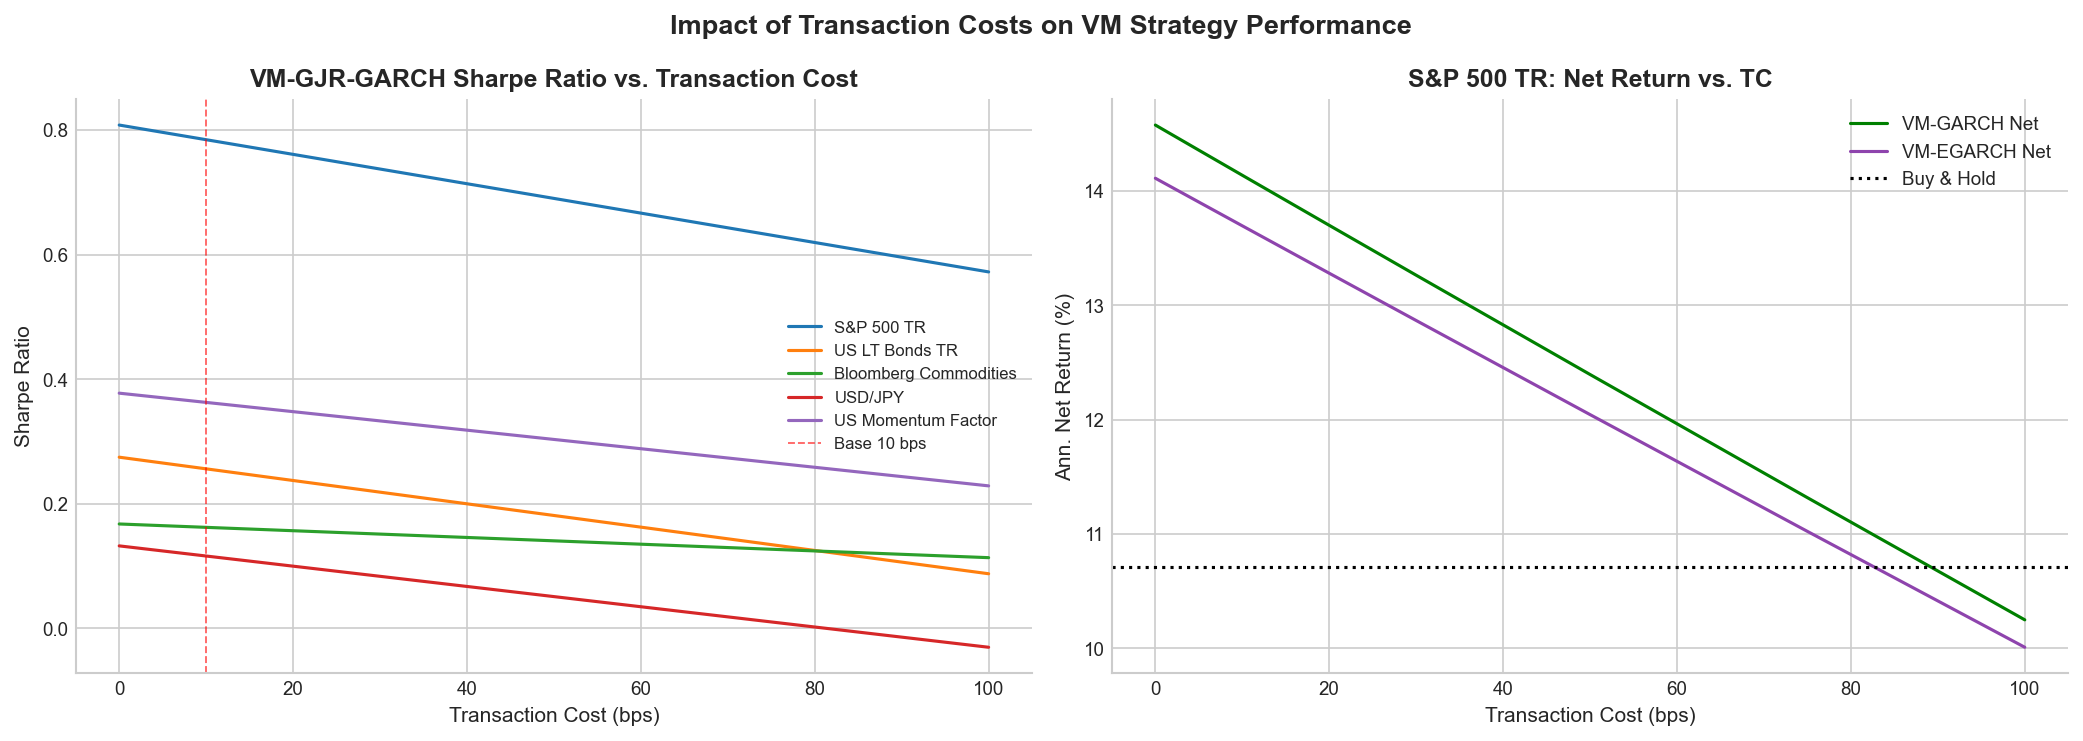
\includegraphics[width=0.88\textwidth]{fig_06_tc_sensitivity.png}
\caption{Impact of transaction costs on VM-GJR-GARCH performance. The breakeven cost for
equities is approximately 64 bps, well above typical institutional execution costs.}
\label{fig:tc}
\end{figure}

\subsection{Turnover Mitigation}

We tested two families of turnover-reduction rules applied to VM GJR-GARCH: threshold bands
(weight updated only when the raw weight differs by more than $b\in\{5\%,10\%,15\%,20\%\}$
from the previous implemented weight) and exponential moving averages of the raw weights
(spans $s\in\{2,3,6,12\}$ months). The full grid is reported in the project notebook;
Table~\ref{tab:tc-mit} summarises the breakeven transaction cost under three rules: the
baseline, the 10\% band, and the EMA span $=3$.

\begin{table}[H]
\centering
\small
\caption{Breakeven Transaction Cost under Mitigation Rules (basis points)}
\label{tab:tc-mit}
\begin{tabular}{lrrr}
\toprule
\textbf{Asset} & \textbf{Baseline} & \textbf{Band 10\%} & \textbf{EMA span 3}\\
\midrule
S\&P 500 TR              & 63.6 & 65.2  & $>100$\\
US LT Bonds TR           & $<0$ & $<0$  & 6.3\\
Bloomberg Commodities    & $<0$ & $<0$  & $<0$\\
USD/JPY                  & 56.6 & 66.1  & $>100$\\
US Momentum Factor       & $>100$ & $>100$ & $>100$\\
\bottomrule
\end{tabular}
\end{table}

\noindent The EMA span~3 rule pushes the breakeven cost above 100~bps for the S\&P 500 and
USD/JPY, an improvement of approximately 60\% over the baseline. For US long-term bonds,
the rule moves the strategy from "never wins" to a positive (if small) breakeven, although
the absolute Sharpe gap is too modest for the result to be practically relevant.
Commodities remain non-viable under every mitigation rule we tested.

\subsection{Leverage Sensitivity}

\begin{table}[H]
\centering
\small
\caption{Leverage Constraint Sensitivity: VM GJR-GARCH Sharpe Ratios}
\label{tab:lev}
\begin{tabular}{lrrrrrr}
\toprule
\textbf{Asset} & \textbf{1.0} & \textbf{1.25} & \textbf{1.5} & \textbf{2.0} & \textbf{3.0} & \textbf{No Cap}\\
\midrule
S\&P 500 TR              & 0.769 & 0.785 & \textbf{0.803} & 0.785 & 0.782 & 0.782\\
US LT Bonds TR           & \textbf{0.289} & 0.281 & 0.259 & 0.256 & 0.256 & 0.256\\
Bloomberg Commodities    & \textbf{0.226} & 0.206 & 0.174 & 0.162 & 0.160 & 0.160\\
USD/JPY                  & 0.071 & 0.091 & 0.105 & \textbf{0.116} & 0.116 & 0.116\\
\bottomrule
\end{tabular}
\end{table}

\noindent For equities, the Sharpe ratio is maximised at a cap of 1.5 (0.803), marginally
above the 2.0 baseline. For bonds and commodities, tighter constraints improve risk-adjusted
performance monotonically: the additional leverage employed by GJR-GARCH on these assets
does not generate sufficient return to compensate for its costs. For USD/JPY, the
relationship is inverse and the Sharpe rises monotonically with the cap up to 2.0. In
practical terms, a 1.5 cap is optimal for equities, 1.0 for bonds and commodities, and 2.0
for USD/JPY.

%% ====================================================================
\section{Summary and Recommendations}

\subsection{Synthesis}

The four conditions identified in Section~1 organise the results clearly: the S\&P 500, the
momentum factor and US LT bonds satisfy the forecastability condition (Mincer-Zarnowitz
$R^2>0.40$); USD/JPY does not. Forecast quality alone does not guarantee economic value, as
commodities have $R^2>0.40$ for GJR-GARCH yet the strategy destroys value. The strategy
benefits assets where the conditional Sharpe ratio is decreasing in volatility, which holds
for the momentum factor in our sample but fails for US long-term bonds (flight-to-quality
dynamic). The breakeven transaction cost is comfortable for equities and FX, but below zero
for bonds and commodities. Critically, only the momentum factor passes the Jobson-Korkie and
bootstrap Sharpe-significance tests at the 5\% level; the equity improvement is suggestive
but not statistically distinguishable from zero. The look-ahead bias, while smaller in our
sample than \citet{liu2019} document for US equity factors (average inflation of $-2.4\%$),
is conceptually fatal because the look-ahead-biased strategy is unimplementable. The
statistical-significance issue is the more durable of the two critiques.

\subsection{Recommendations to the Volatility Management Board}

\textbf{1. Adopt for the momentum factor.} The only statistically significant improvement
in the study (bootstrap $p\in[0.003,0.015]$ for all four models, Fama-French alphas of
7.5--8.7\% per year with $t>2.3$). The point estimate is also the largest: the worst
drawdown is reduced from 61\% to 38\% and the recovery time from a never-recovered position
to 64 months. \textit{Specification:} VM GJR-GARCH or VM RV 6M, EMA smoothing of span 3,
leverage cap of 2.0.

\textbf{2. Adopt for the S\&P 500 with caveats.} The point estimate is favourable
($\Delta SR=+0.126$, drawdown reduced from 51\% to 37\%, recovery time from 37 to 20 months),
the breakeven cost is comfortable ($\approx 64$ bps), and the recession-loss reduction is
6.8 percentage points. However, the Sharpe difference is not statistically significant
($p=0.30$ bootstrap, 95\% CI $[-0.10,+0.35]$) and the Fama-French alpha is not significant
either ($p=0.13$). The Board should adopt this as a probable but not certain Sharpe
improvement. \textit{Specification:} VM GJR-GARCH, EMA span 3 (pushes breakeven $>100$ bps),
leverage cap of 1.5.

\textbf{3. Do not adopt for commodities.} VM Sharpe below Buy and Hold at every positive
cost level (breakeven $<0$ bps). The structural combination of high base volatility, weak
forecast quality, and the secular post-2008 commodity decline leaves the strategy without an
edge. We recommend managing commodity risk through position sizing and cross-asset
diversification rather than through volatility targeting.

\textbf{4. Do not adopt for US long-term bonds.} The flight-to-quality dynamic causes bond
volatility spikes to coincide with positive return episodes; the strategy de-risks at the
worst moments. The Sharpe difference is modestly negative ($\Delta SR=-0.038$) but
consistent across all four models.

\textbf{5. Marginal adoption for USD/JPY.} The improvement is positive but modest
($\Delta SR=+0.076$ for GJR-GARCH) and not statistically significant. Given the weak FX
forecastability, the strategy primarily adds value through drawdown reduction.
\textit{Specification:} VM RV 6M (lowest turnover, highest Sharpe at 0.142) or GJR-GARCH
with Band 15\% mitigation.

\textbf{6. Model selection.} Choose GJR-GARCH as the primary model on three grounds:
superior RMSE and $R^2$ for equities and momentum, an economically interpretable
leverage-effect parameter $\gamma>0$, and lower turnover than RV 1M. EGARCH serves as a
robustness check; the net Sharpe difference between the two GARCH variants is statistically
insignificant on every asset except US LT bonds, where the difference is too small to be
practically relevant.

\textbf{7. Implementation overlays.} An EMA smoothing of span 3 reduces turnover by 30--50\%
with minimal Sharpe sacrifice and, on equities and FX, pushes the breakeven transaction
cost above 100 basis points. We recommend standardising mitigation rules across adopted
strategies to simplify implementation and monitoring.

\textbf{8. Multi-asset implementation.} The equal-weight portfolio of the five GJR-GARCH
variants achieves a Sharpe ratio (0.673) higher than any single-asset variant in our sample,
with a maximum drawdown of 19.5\%. Even if commodities and bonds are not adopted as
standalone overlays, retaining them in a diversified multi-asset portfolio is beneficial
because their volatility-timed returns are nearly orthogonal to the equity and momentum
sleeves.

\subsection{Limitations}

The 2000--2025 sample is dominated by two major crises (2008 and 2020); the strategy's
value-add may differ in a different sample window. Daily rebalancing within each month is
assumed, which may not match real-world operational constraints. The transaction-cost model
is simple (linear, one-way, no market-impact non-linearities). The multi-asset analysis uses
equal weights only; a formal time-varying covariance optimisation is left for future work.
Finally, the Fama-French risk model applies only to the S\&P 500 and the momentum factor;
bond, commodity, and FX assets would require their own multi-factor specifications (term
and default factors, commodity carry and momentum, FX carry and value), which we do not
implement.

%% ====================================================================
\begin{thebibliography}{99}
\bibitem[Andersen et al.(2003)]{andersen2003}
Andersen, T.\ G., Bollerslev, T., Diebold, F.\ X., \& Labys, P.\ (2003).
Modeling and forecasting realized volatility. \textit{Econometrica}, 71(2), 579--625.

\bibitem[Bongaerts et al.(2020)]{bongaerts2020}
Bongaerts, D., Kang, X., \& van Dijk, M.\ (2020).
Conditional volatility targeting. \textit{Financial Analysts Journal}, 76(4), 54--71.

\bibitem[Diebold and Mariano(1995)]{diebold1995}
Diebold, F.\ X., \& Mariano, R.\ S.\ (1995). Comparing predictive accuracy.
\textit{Journal of Business \& Economic Statistics}, 13(3), 253--263.

\bibitem[Frazzini et al.(2018)]{frazzini2018}
Frazzini, A., Israel, R., \& Moskowitz, T.\ J.\ (2018). Trading costs. AQR Working Paper.

\bibitem[Glosten et al.(1993)]{glosten1993}
Glosten, L.\ R., Jagannathan, R., \& Runkle, D.\ E.\ (1993). On the relation between the
expected value and the volatility of the nominal excess return on stocks.
\textit{Journal of Finance}, 48(5), 1779--1801.

\bibitem[Harvey et al.(2018)]{harvey2018}
Harvey, C.\ R., Hoyle, E., Korgaonkar, R., Rattray, S., Sargaison, M., \& Van Hemert, O.\ (2018).
The impact of volatility targeting. \textit{Journal of Portfolio Management}, 45(1), 14--33.

\bibitem[Jobson and Korkie(1981)]{jobson1981}
Jobson, J.\ D., \& Korkie, B.\ M.\ (1981). Performance hypothesis testing with the Sharpe
and Treynor measures. \textit{Journal of Finance}, 36(4), 889--908.

\bibitem[Ledoit and Wolf(2008)]{ledoit2008}
Ledoit, O., \& Wolf, M.\ (2008). Robust performance hypothesis testing with the Sharpe ratio.
\textit{Journal of Empirical Finance}, 15(5), 850--859.

\bibitem[Liu et al.(2019)]{liu2019}
Liu, F., Tang, X., \& Zhou, G.\ (2019). Volatility-managed portfolio: Does it really work?
\textit{Journal of Portfolio Management}, 46(1), 38--51.

\bibitem[Meese and Rogoff(1983)]{meese1983}
Meese, R.\ A., \& Rogoff, K.\ (1983). Empirical exchange rate models of the seventies:
Do they fit out of sample? \textit{Journal of International Economics}, 14(1--2), 3--24.

\bibitem[Memmel(2003)]{memmel2003}
Memmel, C.\ (2003). Performance hypothesis testing with the Sharpe ratio.
\textit{Finance Letters}, 1(1), 21--23.

\bibitem[Mincer and Zarnowitz(1969)]{mincer1969}
Mincer, J., \& Zarnowitz, V.\ (1969). The evaluation of economic forecasts. In J.\ Mincer
(Ed.), \textit{Economic Forecasts and Expectations}, NBER.

\bibitem[Moreira and Muir(2017)]{moreira2017}
Moreira, A., \& Muir, T.\ (2017). Volatility-managed portfolios.
\textit{Journal of Finance}, 72(4), 1611--1644.

\bibitem[Nelson(1991)]{nelson1991}
Nelson, D.\ B.\ (1991). Conditional heteroskedasticity in asset returns: A new approach.
\textit{Econometrica}, 59(2), 347--370.
\end{thebibliography}

\end{document}
